\chapter{Technical Details of Bayesian Optimization}
\label{chapter:bo-indepth}

This chapter provides a more technical insight into Bayesian optimization. We begin by considering acquisition functions from a mathematical perspective, because they form the basis of Bayesian optimization. Next, we show how to extend Bayesian optimization to perform parallel evaluations, work with integer and discrete hyperparameters, and optimize parameters on a logarithmic scale. Finally, we explore the Bayesian optimization algorithm in detail, including some of its numerical properties and issues that can arise when implementing it.

The contents of this chapter deals largely with implementation details and is not necessary to use Bayesian optimization in practice. However, understanding the behavior of integer based hyperparameters, in addition to the overview in \autoref{section:architecture-search}, can prove useful when deciding if a certain hyperparameter makes for a good candidate for automatic tuning using Bayesian optimization.

\section{Acquisition Functions}
\label{section:acq-fn}

An acquisition function is a key component of Bayesian optimization. Together with the GP regression it allows for balancing the exploration-exploitation dilemma in search. The only limitation we impose on the acquisition function is tractability, and possibly continuity, because we need to optimize it. The tractability requirement is mandatory, since without being able to compute the function we could hardly find its maximum. But the continuity requirement is useful given the fact that an acquisition function is often optimized using stochastic gradient optimizers such as L-BFGS.

An intuitive choice for an acquisition function is to maximize the probability
of improving over our currently best achieved value, which is called the
\newterm{probability of improvement}. This can be computed in closed form as
$$
\operatorname{PI}(\vx) = Φ \left( \frac{μ(\vx) - y_{\max}}{σ(\vx)} \right),
$$
where $y_{\max}$ is the maximum value achieved by sampling $f(\vx)$.

A natural extension is the \newterm{expected improvement} (EI) acquisition function,
which is simply the expected improvement over the currently achieved maximum.
We define it as $$\operatorname{EI}(x) = 𝔼[\max(0, f(x) - y_{\max})].$$ At first it might seem that
the expectation would be an intractable integral, but fortunately even this
equation can be computed in closed form as
$$
\operatorname{EI}(x) = Δ(x) + σ(x) φ \left( \frac{Δ(x)}{σ(x)} \right) - |Δ(x)| Φ \left( \frac{Δ(x)}{σ(x)} \right),
$$
where $Δ(x) = μ(x) - y_{\max}$. In practice, the expected improvement shows better results
than the probability of improvement. For more examples of acquisition functions see
\cite{frazier2018tutorial}.

In both of these cases, the next sampling point would be chosen by maximizing
the acquisition function, that is $$x_{\operatorname{next}} = \argmax_x \operatorname{EI}(x)$$ for
the case of expected improvement. This can be performed by utilizing any stochastic optimizer,
such as the commonly chosen L-BFGS with restarts.


\section{Parallel Evaluations}
\label{section:parallel-evaluations}

In practice we might have the means of evaluating $f(\vx)$ at multiple points
in parallel, but the framework we have shown so far only allows for sequential
optimization. A natural extension would be not to optimize with respect
to a single $x_{\operatorname{next}}$, but rather with respect to multiple points. An extension
of EI allowing for optimization with respect to multiple points is called \newterm{parallel expected improvement}.

Unfortunately, maximizing parallel expected improvement has no simple solution \citep{frazier2018tutorial}. A
common solution is the so called \newterm{Constant Liar} approximation, which
chooses $x_{i+1}$ assuming $x_i$ was already chosen, and has the corresponding
value $y_i$ equal to a constant, often chosen to be the expected value of
$f(x_i)$ under the GP posterior.

The Constant Liar approximation enables parallel evaluations by simply
considering the $μ$ prediction for unfinished evaluations as their $y$ value
and consider them part of the dataset $𝓓$.


\section{Integer Hyperparameters}

GP regression by itself does not have the ability to model integer values in $X$ directly as some other models do (e.g. random forests \autoref{chapter:bo}). A common solution, used by \citep{spearmint} and the one we also adopt in this thesis, is to consider all parameters to be real valued and only round after the GP.

In recently published work \cite{integer-valued-gp} the authors show a more principled approach. The effect of rounding causes the model to consider variation and relationships even inside constant-valued regions. A possible downside is that the model could predict values different enough so that the acquisition function would obtain a maximum within a constant region which was already sampled, thus wasting an evaluation. A proposed solution to this problem is to round the appropriate values right before they are processed by the kernel function, such as
$$\kappa'(x_1, x_2) = \kappa(T(x_1), T(x_2)),$$ where $T(x)$ is an identity for real valued elements and a rounding function for integers.

Our implementation however does not use this approach. Instead, we handle the problem explicitly by detecting the pathological cases, as described in \autoref{chapter:software}.

\section{Logarithmic Scaling of Hyperparameters}

When optimizing hyperparameters we might want to distinguish not only real and integer valued ones, but also their scale. Optimizing the number of training epochs or layers is well modelled by a linear scale, but a learning rate is better modelled using a logarithmic scale.

We adopt a simple solution working independently on Bayesian optimization, by simply transforming all of the appropriate values to logarithmic scale before inputting them into the model, and then transforming them back after we get the next sample proposal $x$. Given this approach is completely transparent from the point of the GP regression model, we could just as well perform an arbitrary bijection.


\section{Implementation Details of Bayesian Optimization}
\label{section:bopt-alg}

We now present the algorithm for Bayesian optimization in greater detail compared to \autoref{alg:bopt}. Let $𝓓_n = \{ (\vx_i, y_i), i \in 1:n\}$ denote a set of $n$ samples (evaluations) of the objective function $f$, with $y_i = f(\vx_i)$. Our goal is to pick the next $\vx_{n+1}$ to maximize our chance of finding the optimum quickly, assuming that already enough points were evaluated for us to fit the GP. \autoref{alg:bopt-detailed} shows one iteration of Bayesian optimization as it proposes $\vx_{n+1}$.

\begin{algorithm}
	\label{alg:bopt-detailed}
	\DontPrintSemicolon
	\SetAlgoLined
	Let $\mX$ be the matrix of all $\vx_i$, and $\vy$ be a column vector of all $y_i$. \;
	Maximize the kernel log-likelihood $$p(\mX) = -\frac{1}{2}\vy \mK^{-1}\vy - \frac{1}{2} \log \det \mK - \frac{N}{2} \log (2 π),$$ where $\mK = \kappa(\mX, \mX)$, by tuning the kernel hyperparameters. \;
	Maximize the acquisition function $A(\mX, \vy, \mathcal{G}\mathcal{P})$ as a function of the GP using the kernel hyperparameters obtained in the previous step. \;
	Sample $y_{n+1} = f(\vx)$, where $\vx = \argmax A(\mX, \vy, \mathcal{G}\mathcal{P})$. \;
	Add $y_{n+1}$ to the dataset as $𝓓_{i+1} = 𝓓_i \cup (\vx_{i+1}, y_{i+1})$.
	\caption{Bayesian Optimization with implementation details.}
\end{algorithm}

While this algorithm explains how Bayesian optimization works, there are a few cases where numerical issues can arise, and we point them out next.

Firstly, the quadratic form $\vy \mK^{-1} \vy$ does not need to be computed using a matrix inversion procedure, which can be numerically unstable and requires more intermediate computation (see \cite{cholesky-inverse-krishnamoorthy2013matrix} for details). In general, consider the equation $\mA \vx = \vb$. We can rewrite it to $\vx = \mA^{-1} \vb$ for an invertible matrix $\mA$. A naive solution would compute the inverse and then the multiplication to get $\inv(\mA) \vb$, but because we do not actually need the inverse itself, we can solve for $\mA^{-1} \vb$ directly using a \inlinecode{solve} procedure \citep{numpy}.

Because the $\mK$ matrix is a covariance matrix, we also know it is positive definite. This allows us to compute its Cholesky factorization $\mL = \chol(\mK)$, and then apply a procedure for \inlinecode{solve} directly on the factorized matrix $\mL$ (in TensorFlow available as \inlinecode{tf.linalg.cholesky\_solve}).

Having just computed the Cholesky factorization we can re-use it in the second expression of the marginal log-likelihood, that is the $\log \det \mK$, since
\begin{align}
\log \det \mK &= \log \det(\mL^T \mL) = \log(\det(\mL^T) \cdot \det(\mL)) = \\
&= 2 \cdot \log \det \mL = 2 \cdot \log \prod \diag \mL = 2 \cdot \sum \log \diag \mL.
\end{align}
This form allows computing the determinant, which usually takes $𝓞(n^3)$, in just linear time, by re-using the work already performed during the Cholesky factorization produced in the previous step.

Another interesting note, discovered by our initial custom implementation, and confirmed in the implementation of the GPy \citep{gpy2014} library, is that when computing a Cholesky factorization of a covariance matrix computed on real world data, it often fails for numerical reasons, and requires additional noise to be added to the diagonal to improve stability. What GPy does internally is to iteratively increase the amount of noise, up until some threshold, to make sure the factorization succeeds, while not adding excessive noise when not needed.

Lastly, the optimization procedures themselves used for maximizing the kernel log-likelihood and acquisition function can be sensitive. Our initial implementation in SciPy and TensorFlow demonstrated quite different results based on the type of the optimizer (SGD, Adam, L-BFGS), and its meta-parameters, such as the number of restarts, stop tolerance criterion, learning rates, etc. These problems, along with many numerical issues encountered along the way, contributed to the choice of using GPy for the final implementation. We outline a few more reasons in \autoref{section:gpy}.


\section{Priors on Kernel Parameters}
\label{section:priors-on-kernel-params}

One of the benefits of the GP regression model is that it is very flexible. Unlike parametric models, such as linear regression, it can fit arbitrarily complex predictions of the data. This flexibility is dictated by the choice of a kernel function, which determines individual covariances between every pair of points. As we have shown earlier (see \autoref{section:kernels}), the kernels themselves have hyperparameters which greatly affect the behavior of the model. Even though it is theoretically possible to set the kernel parameters by hand, as it could be done if we knew some properties of the objective function, we cannot take this approach when fitting arbitrary samples from the loss landscape of a neural network. Instead, we take a principled approach using statistics and optimize the kernel parameters to maximize the likelihood of the data, specifically by using maximum likelihood estimation (MLE).

Unfortunately, because MLE is a point estimate, it is prone to overfitting. In our particular case of using a flexible non-parametric model we can run into severe case of overfitting. In theory, some argue (see \citep{williams2006gaussian}) that when the likelihood function is multi-modal, there are usually multiple interpretations to the data, and each mode maps to an intuitive interpretation. We have not found this to be true on more complex datasets, as those sampled from the objective function of neural networks models, and very often the MLE ends up choosing a model with extremely high capacity, as shown in \autoref{figure:overfitting-gp}.

\begin{figure}
	\begin{center}
		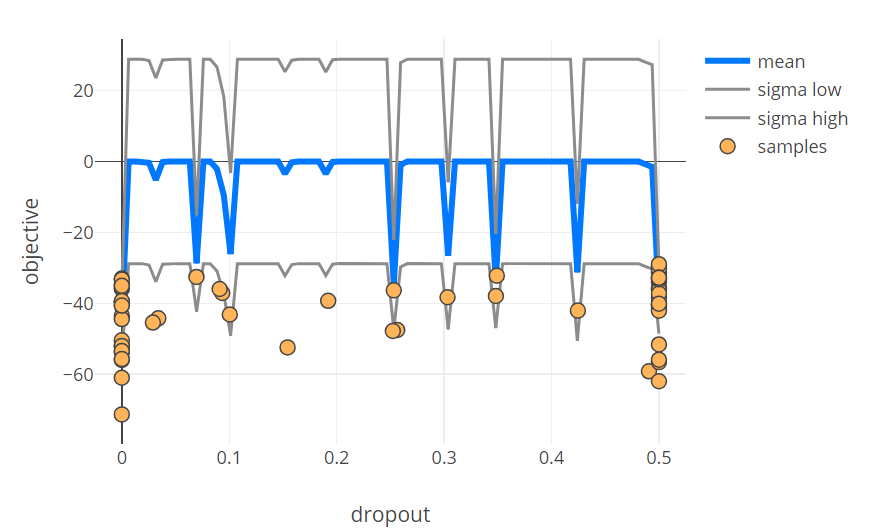
\includegraphics[width=1.0\textwidth]{images/overfitting-gp.png}
		\caption{GP regression with a very low value for the lengthscale kernel parameter. Since the scale parameter is low, the $x$ axis ends up being \emph{stretched out}, and each data point becomes independent, that is their covariance is low. As a result, the model is free to try to fit almost every data point independently on the others, and its predictions become uninformative.}
		\label{figure:overfitting-gp}
	\end{center}
\end{figure}

A common solution to the overfitting problem of MLE is to introduce a prior distribution $p(w)$ on the parameters $w$, and then instead of maximizing the likelihood $p(x|w)$ we would maximize the posterior distribution $p(w | x) \propto p(x | w) p(w)$. This approach is commonly called the maximum a posteriori (MAP) estimate, and is frequently employed in machine learning models as a way of reducing overfitting. For example, in the case of linear regression, the standard least squares solution corresponds to maximizing the likelihood of the data using MLE, or equivalently minimizing the mean squared error between the predictions and the labels. A probabilistic extension of linear regression, which introduces a Gaussian prior on the weights, is called a Ridge regression (or L2 regularization), and corresponds to computing the MAP estimate of the parameters, or equivalently minimizing the mean squared error with an additional weight decay term.

In the ideal case, we would either marginalize over the parameters, or take a fully Bayesian approach and compute the posterior $p(w | x)$. Unfortunately, in many cases including ours, the marginalization becomes intractable due to the normalization constant given by the evidence term $p(x)$. The MAP estimate is a practical compromise between the frequentist point estimate using MLE, and a fully Bayesian treatment. Because we only need to compute the $\argmax$ of the posterior, we can optimize it without computing the normalization term $p(x)$, given $\argmax$ being invariant to scaling by a constant. The MAP estimate is then simply computed as $$ \argmax_w p(x|w) p(w), $$ where in our case $w$ represents the kernel parameters, as well as the constant for Gaussian noise in each sample.

As with any Bayesian method, the choice of a prior is of great importance. If we were to choose a uniform prior, computing the MAP estimate would be equivalent to computing the MLE with constrained optimization on the support of the uniform distribution. In practice, we could take a conservative step and choose a non-informative prior, which would still act as regularization, and possibly help with overfitting as compared to computing a bare MLE estimate. An example of such prior is the $\operatorname{Gamma}(1.0, 0.001)$ distribution shown in \autoref{figure:gamma-prior}, because its support are positive real numbers, and both the variance and the lengthscale of the kernel are also defined only for positive real numbers.

In our experiments described in \autoref{chapter:experiments}, we show a few cases where the choice of an uninformative prior leads to poor model behavior. The common cause if the model choosing a small lengthscale for hyperparameters with high range of values, as shown previously in \autoref{figure:overfitting-gp}. Because the process of Bayesian optimization is built on top of the regression model, it can become problematic when the model considers most of the search space as constant regions with only a few peaks at the sampled data points.

A possible solution to this problem is to abandon the idea of non-informative priors and instead adopt the approach often called Empirical Bayes \citep{murphy2012machine}, where the parameters of the prior distribution are estimated from the data themselves. Choosing between a non-informative prior and estimating the parameters from data is a principal problem that does not have a definitive answer.

With our motivations being largely driven by practical applications rather than theoretical purity, we do estimate the prior parameters from data in some visualizations (see \autoref{section:visualizations}) to avoid pathological cases and provide more useful user experience. We also show comparisons between the non-informative priors and the Empirical Bayes approach in the GP regression model used when computing the acquisition function, as compared to only in visualizations, in \autoref{section:experiments-empirical-bayes}. Unfortunately, because some experiments were very computationally intensive (some over a thousand GPU-hours), we do not provide a full ablation analysis.

\begin{figure}
	\begin{center}
		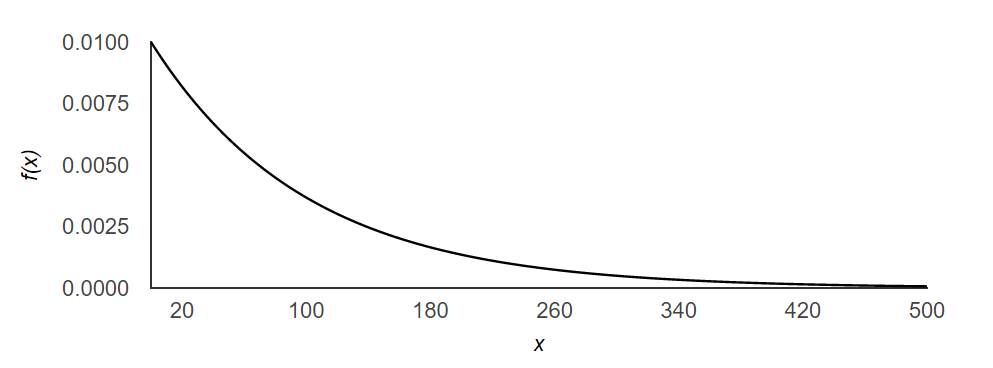
\includegraphics[width=1.0\textwidth]{images/gamma-prior.png}
		\caption{An example of a prior distribution defined as $\operatorname{Gamma}(1.0, 0.001)$ with support over positive real numbers.}
		\label{figure:gamma-prior}
	\end{center}
\end{figure}

